\documentclass[12pt]{article}
\usepackage[utf8]{inputenc}
\usepackage[spanish]{babel}
\usepackage{amsmath}
\usepackage{amsthm}
\usepackage{hyperref}
\usepackage{graphicx}
\usepackage{color}
\usepackage{float}
\usepackage{multicol}
\usepackage{enumerate}
\usepackage{anyfontsize}
\usepackage{anysize}
\usepackage{tikz}
\usepackage{siunitx}
\usepackage{gensymb}
\usetikzlibrary{arrows.meta, positioning}
\setlength{\parskip}{1em}
\spanishdecimal{.}


\title{Ejercicios de repaso \vspace{-2cm}}
\author{}
\date{ }

%--------------------------------------------------------------------
\newcounter{choice}
\renewcommand\thechoice{\Alph{choice})}
%\newcommand\choicelabel{\thechoice.}
\newcommand\choicelabel{\thechoice}

\newenvironment{choices}%
  {\list{\choicelabel}%
     {\usecounter{choice}\def\makelabel##1{\hss\llap{##1}}%
       \settowidth{\leftmargin}{W.\hskip\labelsep\hskip 2.5em}%
       \def\choice{%
         \item
       } % choice
       \labelwidth\leftmargin\advance\labelwidth-\labelsep
       \topsep=0pt
       \partopsep=0pt
     }%
  }%
  {\endlist}

\newenvironment{oneparchoices}%
  {%
    \setcounter{choice}{0}%
    \def\choice{%
      \refstepcounter{choice}%
      \ifnum\value{choice}>1\relax
        \penalty -50\hskip 1em plus 1em\relax
      \fi
      \choicelabel
      \nobreak\enskip
    }% choice
    % If we're continuing the paragraph containing the question,
    % then leave a bit of space before the first choice:
    \ifvmode\else\enskip\fi
    \ignorespaces
  }%
  {}
%----------------------------------------------------------

\begin{document}
\maketitle
\fontsize{14}{14}\selectfont

Escribe la medidas de los ángulos marcados con las letras en la siguiente figura. Justifica tus respuestas.
\begin{figure}[H]
    \centering
    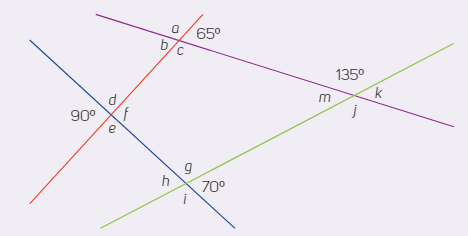
\includegraphics[scale=1]{Imagenes/Angulos_02.png}
\end{figure}
\noindent
\begin{multicols}{2}
$\measuredangle \, a = $ \, \rule{2cm}{0.1mm} \\
$\measuredangle \, b = $ \, \rule{2cm}{0.1mm} \\
$\measuredangle \, c = $ \, \rule{2cm}{0.1mm} \\
$\measuredangle \, d = $ \, \rule{2cm}{0.1mm} \\
$\measuredangle \, e = $ \, \rule{2cm}{0.1mm} \\
$\measuredangle \, f = $ \, \rule{2cm}{0.1mm} \\
\columnbreak
\\
$\measuredangle \, g = $ \, \rule{2cm}{0.1mm} \\
$\measuredangle \, h = $ \, \rule{2cm}{0.1mm} \\
$\measuredangle \, i = $ \, \rule{2cm}{0.1mm} \\
$\measuredangle \, j = $ \, \rule{2cm}{0.1mm} \\
$\measuredangle \, k = $ \, \rule{2cm}{0.1mm} \\
$\measuredangle \, m = $ \, \rule{2cm}{0.1mm}
\end{multicols}

\newpage
A los ángulos que se fomran entre dos rectas y una \textbf{transversal} se les denomina en términos de las relaciones que guardan entre sí, ya sea que las rectas sean paralelas o no.
\begin{figure}[H]
    \centering
    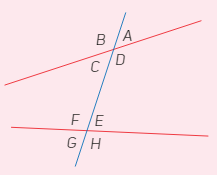
\includegraphics[scale=1.5]{Imagenes/Angulos_03.png}
\end{figure}
\begin{itemize}
\item Los ángulos \textbf{alternos internos} son aquellos que están en la región comprendida entre las rectas (región interior) y lados opuestos de la transversal.
\item Los ángulos \textbf{alternos externos} son los que están en la región exterior a las rectas y en lados opuestos de la transversal.
\item Se llaman ángulos \textbf{colaterales externos} a los que están del mismo lado de la transversal y en la región exterior a las rectas.
\item Los ángulos \textbf{correspondientes} son aquellos que están del mismo lado de la transversal, pero uno de ellos es interno y el otro externo. 
\end{itemize}
Identificar un ángulo normalmente se hace por parejas de ángulos.
\\
\noindent
Identifica las parejas de ángulos y escribe su letra en el renglón que corresponda.
\begin{multicols}{2}
\begin{enumerate}[label=\alph*)]
\item Alternos internos. \rule{2cm}{0.1mm}
\item Alternos externos. \rule{2cm}{0.1mm}
\item Colaterales internos. \rule{2cm}{0.1mm}
\columnbreak
\item Colaterales externos. \rule{2cm}{0.1mm}
\item Correspondientes. \rule{2cm}{0.1mm}
\end{enumerate}
\end{multicols}

\end{document}